
%  ========== PREAMBLE ==========

\documentclass[11pt]{article}

% -= Packages =-

\usepackage[top=1in,bottom=1in,left=1in,right=1in,paper=a4paper]{geometry}
\usepackage{graphicx,float}
\usepackage{hyperref}
\usepackage{tocloft}
\usepackage[immediate]{silence}
\WarningFilter[temp]{latex}{Command} % silence the warning
\usepackage{sectsty}
\DeactivateWarningFilters[temp] % So nothing unrelated gets silenced
\usepackage[most]{tcolorbox}
\usepackage{textcomp}
\usepackage{amsmath,amsfonts,amssymb,amsthm,mathtools,gensymb}
\usepackage{hyperref}
\usepackage{tikz}
\usepackage{titling}
\usepackage{lipsum}
\usepackage{mathtools}
\usepackage{enumitem}
\usepackage[utf8]{inputenc}
\usepackage[titletoc,title]{appendix}
\usepackage{xcolor}
\usepackage[twoside]{fancyhdr}
\usepackage[parfill]{parskip}
\usepackage{multicol}
\usepackage{pgfplots}
\pgfplotsset{compat=1.15}
\usepackage{mathrsfs}
\usetikzlibrary{arrows}
\usepackage{fontawesome5}
\usepackage{titlesec}

\usetikzlibrary{arrows.meta, decorations.pathreplacing,calc}

\makeatletter % disable the runtime redefinitions
\let\SS@makeulinesect\relax
\let\SS@makeulinepartchap\relax
\makeatother


% -= Settings =-

\pagestyle{fancy}
\allsectionsfont{\bfseries\sffamily}

\graphicspath{ {./images/} }

\hypersetup{
    colorlinks,
    citecolor=black,
    filecolor=black,
    linkcolor=purple,
    urlcolor=blue
}


\renewcommand{\baselinestretch}{1.5}
\newcommand{\qedblack}{$\hfill\blacksquare$}

\newcommand{\divides}{\mid}
\newcommand{\notdivides}{\nmid}

\DeclareMathOperator{\ord}{ord}

\DeclarePairedDelimiter\abs{\lvert}{\rvert}%
\DeclarePairedDelimiter\norm{\lVert}{\rVert}%

\renewcommand{\footrulewidth}{0.45pt}
\renewcommand{\headrulewidth}{0.45pt}
\definecolor{bbe}{HTML}{000000}
\definecolor{headerbg}{RGB}{0, 0, 0} 
\definecolor{headertext}{RGB}{255, 250, 240}
\definecolor{mahdarkblue}{HTML}{1e3f66}
\definecolor{mahdarknavy}{HTML}{254a6d}
\definecolor{mahnavy}{HTML}{2e5984}
\definecolor{mahblue}{HTML}{528aae}
\definecolor{mahlightblue}{HTML}{73a5c6}
\definecolor{mahsky}{HTML}{91bad6}
\definecolor{mahturquoise}{HTML}{5f8998}
\setlength{\headheight}{21pt}


% -= Theorem Environments =-

\newtcolorbox[auto counter,number within=section,number format=\arabic]{definition}[1][]{
            colback=mahdarkblue!10!white,enhanced,
            title={\textbf{\faBook\ \ Định nghĩa~\thetcbcounter}},
            attach boxed title to top left={xshift=-4mm},
            boxrule=0pt,
            after skip=1cm,before skip=1cm,right skip=0cm,
            breakable,fonttitle=\sffamily,
            toprule=0pt,bottomrule=0pt,rightrule=0pt,leftrule=4pt,
            arc=0mm,
            skin=enhancedlast jigsaw,
            sharp corners,
            colframe=mahdarkblue,colbacktitle=mahdarkblue!90!white,
            boxed title style={
                frame code={
                    \fill[mahdarkblue!90!white](frame.south west)--(frame.north west)--(frame.north east)--([xshift=3mm]frame.east)--(frame.south east)--cycle;
                    \draw[line width=1mm,mahdarkblue!90!white]([xshift=2mm]frame.north east)--([xshift=5mm]frame.east)--([xshift=2mm]frame.south east);
                    \draw[line width=1mm,mahdarkblue!90!white]([xshift=5mm]frame.north east)--([xshift=8mm]frame.east)--([xshift=5mm]frame.south east);
                    \fill[mahdarkblue!80!white](frame.south west)--+(4mm,-2mm)--+(4mm,2mm)--cycle;
                }
            }
}

\newtcolorbox[auto counter,number within=section,number format=\arabic]{theorem}[1][]{
            colback=mahdarknavy!10!white,enhanced,
            title={\textbf{\faPen\ \ Định lí~\thetcbcounter}},
            attach boxed title to top left={xshift=-4mm},
            boxrule=0pt,
            after skip=1cm,before skip=1cm,right skip=0cm,
            breakable,fonttitle=\sffamily,
            toprule=0pt,bottomrule=0pt,rightrule=0pt,leftrule=4pt,
            arc=0mm,
            skin=enhancedlast jigsaw,
            sharp corners,
            colframe=mahdarknavy,colbacktitle=mahdarknavy!90!white,
            boxed title style={
                frame code={
                    \fill[mahdarknavy!90!white](frame.south west)--(frame.north west)--(frame.north east)--([xshift=3mm]frame.east)--(frame.south east)--cycle;
                    \draw[line width=1mm,mahdarknavy!90!white]([xshift=2mm]frame.north east)--([xshift=5mm]frame.east)--([xshift=2mm]frame.south east);
                    \draw[line width=1mm,mahdarknavy!90!white]([xshift=5mm]frame.north east)--([xshift=8mm]frame.east)--([xshift=5mm]frame.south east);
                    \fill[mahdarknavy!80!white](frame.south west)--+(4mm,-2mm)--+(4mm,2mm)--cycle;
                }
            }
}

\newtcolorbox[auto counter,number within=section,number format=\arabic]{property}[1][]{
            colback=mahnavy!10!white,enhanced,
            title={\textbf{\faBookmark\ \ Tính chất~\thetcbcounter}},
            attach boxed title to top left={xshift=-4mm},
            boxrule=0pt,
            after skip=1cm,before skip=1cm,right skip=0cm,
            breakable,fonttitle=\sffamily,
            toprule=0pt,bottomrule=0pt,rightrule=0pt,leftrule=4pt,
            arc=0mm,
            skin=enhancedlast jigsaw,
            sharp corners,
            colframe=mahnavy,colbacktitle=mahnavy!90!white,
            boxed title style={
                frame code={
                    \fill[mahnavy!90!white](frame.south west)--(frame.north west)--(frame.north east)--([xshift=3mm]frame.east)--(frame.south east)--cycle;
                    \draw[line width=1mm,mahnavy!90!white]([xshift=2mm]frame.north east)--([xshift=5mm]frame.east)--([xshift=2mm]frame.south east);
                    \draw[line width=1mm,mahnavy!90!white]([xshift=5mm]frame.north east)--([xshift=8mm]frame.east)--([xshift=5mm]frame.south east);
                    \fill[mahnavy!80!white](frame.south west)--+(4mm,-2mm)--+(4mm,2mm)--cycle;
                }
            }
}

\newtcolorbox[auto counter,number format=\arabic]{problem}[1][]{
            colback=mahblue!10!white,enhanced,
            title={\textbf{\faFile*\ \ Problem~\thetcbcounter}},
            attach boxed title to top left={xshift=-4mm},
            boxrule=0pt,
            after skip=1cm,before skip=1cm,right skip=0cm,
            breakable,fonttitle=\sffamily,
            toprule=0pt,bottomrule=0pt,rightrule=0pt,leftrule=4pt,
            arc=0mm,
            skin=enhancedlast jigsaw,
            sharp corners,
            colframe=mahblue,colbacktitle=mahblue!90!white,
            boxed title style={
                frame code={
                    \fill[mahblue!90!white](frame.south west)--(frame.north west)--(frame.north east)--([xshift=3mm]frame.east)--(frame.south east)--cycle;
                    \draw[line width=1mm,mahblue!90!white]([xshift=2mm]frame.north east)--([xshift=5mm]frame.east)--([xshift=2mm]frame.south east);
                    \draw[line width=1mm,mahblue!90!white]([xshift=5mm]frame.north east)--([xshift=8mm]frame.east)--([xshift=5mm]frame.south east);
                    \fill[mahblue!80!white](frame.south west)--+(4mm,-2mm)--+(4mm,2mm)--cycle;
                }
            }
}

\newtcolorbox[auto counter,number within=section,number format=\arabic]{problemme}[1][]{
            colback=mahblue!10!white,enhanced,
            title={\textbf{\faFile*\ \ Problem statement}},
            attach boxed title to top left={xshift=-4mm},
            boxrule=0pt,
            after skip=1cm,before skip=1cm,right skip=0cm,
            breakable,fonttitle=\sffamily,
            toprule=0pt,bottomrule=0pt,rightrule=0pt,leftrule=4pt,
            arc=0mm,
            skin=enhancedlast jigsaw,
            sharp corners,
            colframe=mahblue,colbacktitle=mahblue!90!white,
            boxed title style={
                frame code={
                    \fill[mahblue!90!white](frame.south west)--(frame.north west)--(frame.north east)--([xshift=3mm]frame.east)--(frame.south east)--cycle;
                    \draw[line width=1mm,mahblue!90!white]([xshift=2mm]frame.north east)--([xshift=5mm]frame.east)--([xshift=2mm]frame.south east);
                    \draw[line width=1mm,mahblue!90!white]([xshift=5mm]frame.north east)--([xshift=8mm]frame.east)--([xshift=5mm]frame.south east);
                    \fill[mahblue!80!white](frame.south west)--+(4mm,-2mm)--+(4mm,2mm)--cycle;
                }
            }
}

\newtcolorbox[auto counter,number format=\arabic]{exproblem}[1][]{
            colback=mahblue!10!white,enhanced,
            title={\textbf{\faFile*\ \ Ví dụ~\thetcbcounter}},
            attach boxed title to top left={xshift=-4mm},
            boxrule=0pt,
            after skip=1cm,before skip=1cm,right skip=0cm,
            breakable,fonttitle=\sffamily,
            toprule=0pt,bottomrule=0pt,rightrule=0pt,leftrule=4pt,
            arc=0mm,
            skin=enhancedlast jigsaw,
            sharp corners,
            colframe=mahblue,colbacktitle=mahblue!90!white,
            boxed title style={
                frame code={
                    \fill[mahblue!90!white](frame.south west)--(frame.north west)--(frame.north east)--([xshift=3mm]frame.east)--(frame.south east)--cycle;
                    \draw[line width=1mm,mahblue!90!white]([xshift=2mm]frame.north east)--([xshift=5mm]frame.east)--([xshift=2mm]frame.south east);
                    \draw[line width=1mm,mahblue!90!white]([xshift=5mm]frame.north east)--([xshift=8mm]frame.east)--([xshift=5mm]frame.south east);
                    \fill[mahblue!80!white](frame.south west)--+(4mm,-2mm)--+(4mm,2mm)--cycle;
                }
            }
}

\newtcolorbox[auto counter,number within=section,number format=\arabic]{corollary}[1][]{
            colback=mahlightblue!10!white,enhanced,
            title={\textbf{\faHandPointRight[regular] \ \ Hệ quả \thetcbcounter}},
            boxrule=0pt,
	    frame hidden,
            breakable,fonttitle=\sffamily,
            arc=0mm,
            sharp corners,
            detach title,
            before upper = \tcbtitle\par\smallskip,
            colframe=mahlightblue,coltitle=mahlightblue!85!black,
            borderline west = {1mm}{0pt}{mahlightblue!85!black},
            segmentation style={solid, mahlightblue!85!black}
}

\newtcolorbox[auto counter,number format=\arabic]{lemma}[1][]{
            colback=mahlightblue!10!white,enhanced,
            title={\textbf{\faBook \ \ Bổ đề}},
            boxrule=0pt,
	    frame hidden,
            breakable,fonttitle=\sffamily,
            arc=0mm,
            sharp corners,
            detach title,
            before upper = \tcbtitle\par\smallskip,
            colframe=mahlightblue,coltitle=mahlightblue!85!black,
            borderline west = {1mm}{0pt}{mahlightblue!85!black},
            segmentation style={solid, mahlightblue!85!black}
}

\newtcolorbox[auto counter,number format=\arabic]{claim}[1][]{
            colback=mahturquoise!10!white,enhanced,
            title={\textbf{\faExclamation \ \ Claim --- \ }},
            boxrule=0pt,
	    frame hidden,
            breakable,fonttitle=\sffamily,
            arc=0mm,
            sharp corners,
            detach title,
            before upper = \tcbtitle,
            colframe=mahturquoise,coltitle=mahturquoise!85!black,
            borderline west = {1mm}{0pt}{mahturquoise!85!black},
            segmentation style={solid, mahturquoise!85!black}
}

\newtcolorbox[auto counter,number format=\arabic]{remark}[1][]{
            colback=mahsky!10!white,enhanced,
            title={\textbf{\faExclamation \ \ Remark --- \ }},
            boxrule=0pt,
	    frame hidden,
            breakable,fonttitle=\sffamily,
            arc=0mm,
            sharp corners,
            detach title,
            before upper = \tcbtitle,
            colframe=mahsky,coltitle=mahsky!85!black,
            borderline west = {1mm}{0pt}{mahsky!85!black},
            segmentation style={solid, mahsky!85!black}
}

\newtcolorbox[auto counter,number format=\arabic]{motivation}[1][]{
            colback=mahlightblue!10!white,enhanced,
            title={\textbf{\faQuestion \ \ Motivation}},
            boxrule=0pt,
	    frame hidden,
            breakable,fonttitle=\sffamily,
            arc=0mm,
            sharp corners,
            detach title,
            before upper = \tcbtitle\par\smallskip,
            colframe=mahlightblue,coltitle=mahlightblue!85!black,
            borderline west = {1mm}{0pt}{mahlightblue!85!black},
            segmentation style={solid, mahlightblue!85!black}
}

\newenvironment{solution}[1][Solution]{%
  \proof[\normalfont \faPenNib \hspace{0.2cm} \ttfamily \scshape \large #1]%
}{\(\hfill \blacksquare\){\parfillskip0pt\par}}

\theoremstyle{definition}
\newtheorem{exercise}{Problem}

\newcommand{\boom}{\vspace{0.25cm}}


% -= Header + Title =-

% Header

\fancyhead[RO]{\footnotesize \thepage}
\fancyhead[RE]{\footnotesize \textsc{VMO 2014 Solution Notes}}
\fancyhead[LE]{\footnotesize \thepage}
\fancyhead[LO]{\footnotesize \scshape Mark Nguyen}
\fancyfoot{}

\renewcommand{\footrulewidth}{0pt}

% Section title

\makeatletter
\titleformat{\section}
  {\normalfont\Large\bfseries\sffamily}{\color{purple}\S\thesection}{1em}{}
\titleformat{\subsection}
  {\normalfont\large\bfseries\sffamily}{\color{purple}\S\thesubsection}{1em}{}
\titleformat{\subsubsection}
  {\normalfont\normalsize\bfseries\ttfamily}{\color{purple}\S\thesubsubsection}{1em}{}
\makeatother
  

\renewcommand{\cfttoctitlefont}{\hfill\bfseries\LARGE}
\renewcommand{\cftaftertoctitle}{\hfill\hspace{-1cm}}

\title{\textbf{\Huge VMO 2014 Solution Notes}}
\author{\LARGE \textsc{Mark Nguyen}}
\date{\sffamily\today}

\begin{document}

\maketitle

\begin{abstract}
    This document compiles my solutions and best attempts for the 2014 Vietnamese Mathematical Olympiad. While I originally considered writing in Vietnamese, I chose English to make it accessible to a wider audience and to refine my language skills. All content is authored and maintained by me. Comments and corrections are welcome.
\end{abstract}

\tableofcontents

\newpage

\section{Problems}

    \subsection*{Day 1}

        \begin{exercise}
            Given two sequences \((x_n)_{n=1}^{+\infty}\) and \((y_n)_{n=1}^{+\infty}\) of positive real numbers, defined by \(x_1 = 1\), \(y_1 = \sqrt{3}\), and for all positive integers \(n\),
            \[\begin{cases}
                x_{n+1}y_{n+1} - x_n = 0 \\
                x_{n+1}^2 + y_n = 2
            \end{cases}.\]
            Prove that \((x_n)_{n=1}^{+\infty}\) and \((y_n)_{n=1}^{+\infty}\) converges, then find \(\lim\limits_{n \to +\infty} x_n\) and \(\lim\limits_{n \to +\infty} y_n\).
        \end{exercise}
    
        \boom
    
        \begin{exercise}
            Prove that for all positive integers \(n\), the polynomial
            \[P(x) = (x^2 - 7x + 6)^{2n} + 13\]
            cannot be written as the product of \(n + 1\) non-constant polynomials with integer coefficients.
        \end{exercise}
    
        \boom
    
        \begin{exercise}
            Given a regular 103-sided polygon with 79 vertices colored red and the remaining vertices colored blue. Denote \(A\) as the number of pairs of adjacent red vertices, and \(B\) as the number of pairs of adjacent blue vertices.
            \begin{enumerate}
                \item[(a)] Find all possible values of \((A,B)\).
                \item[(b)] Two ways of colorings of the polygon are called \emph{similar} if one of them can be obtained from another through rotation at the circumcenter of the regular polygon. Determine the number of pairwise non-similar colorings of the polygon satisfying \(B = 14\).
            \end{enumerate}
        \end{exercise}
    
        \boom
    
        \begin{exercise}
            Let \(ABC\) be an acute and scalene triangle (\(AB < AC)\)) with circumcircle \((O)\). Let \(I\) be the midpoint of arc \(BC\) not containing \(A\) of circle \((O)\). Let \(K\) be a point on \(AC\) (\(K \neq C\)) such that \(IK = IC\). Line \(BK\) intersects \((O)\) at \(D\) (\(D \neq B\)) and intersects \(AI\) at \(E\). \(DI\) intersects \(AC\) at \(F\).
            \begin{enumerate}
                \item[(a)] Prove that \(EF = \dfrac{BC}{2}\).
                \item[(b)] Let \(M\) be a point on \(DI\) satisfies \(CM\) is parallel to \(AD\). Line \(KM\) intersects \(BC\) at \(N\), and the circumcircle of triangle \(BKN\) intersects \((O)\) at \(P\) (\(P \neq B\)). Prove that \(PK\) passes through the midpoint of segment \(AD\).
            \end{enumerate}
        \end{exercise}

    \newpage
    
    \subsection*{Day 2}

        \begin{exercise}
            Given a fixed circle \((O)\), \(B\) and \(C\) are fixed points on \((O)\), and \(A\) is a moving point on \((O)\) such that \(ABC\) is an acute, scalene triangle. Point \(M\), \(N\) lies on ray \(AB\), \(AC\) respectively, such that \(MA = MC\) and \(NA = NB\). Let \(P\) be the intersection of circles \((AMN)\) and \((O)\), and \(Q\) be the intersection of lines \(MN\) and \(BC\).
            \begin{enumerate}
                \item[(a)] Prove that \(A\), \(P\), and \(Q\) are collinear.
                \item[(b)] Let \(D\) be the midpoint of segment \(BC\), \(K\) be the intersection of circles \((M;MA)\) and \((N;NA)\) (\(K \neq A\)). The line passing through \(A\) perpendicular to \(AK\) intersects \(BC\) at \(E\). The circumcircle of triangle \(ADE\) intersects \((O)\) at \(F\) (\(F \neq A\)). Prove that \(AF\) passes through a fixed point as \(A\) moves on \((O)\).
            \end{enumerate}
        \end{exercise}
    
        \boom
    
        \begin{exercise}
            Let \(x\), \(y\), and \(z\) be positive real numbers. Find the maximum value of the expression
            \[\frac{x^3y^4z^3}{(x^4 + y^4)(xy + z^2)^3} + \frac{y^3z^4x^3}{(y^4 + z^4)(yz + x^2)^3} + \frac{z^3x^4y^3}{(z^4 + x^4)(zx + y^2)^3}.\]
        \end{exercise}
    
        \boom
    
        \begin{exercise}
            Find all ordered sets of 2014 rational numbers, not necessarily distinct, such that if an arbitrary number in the set is removed, one can always partite the remaining 2013 numbers into 3 sets, such that each set has exactly 671 elements, and the product of all elements in each sets are all equal.
        \end{exercise}

    \newpage

\section{Solutions}

    \subsection{Solutions for Day 1}

        \begin{problem}
            Given two sequences \((x_n)_{n=1}^{+\infty}\) and \((y_n)_{n=1}^{+\infty}\) of positive real numbers, defined by \(x_1 = 1\), \(y_1 = \sqrt{3}\), and for all positive integers \(n\),
            \[\begin{cases}
                x_{n+1}y_{n+1} - x_n = 0 \\
                x_{n+1}^2 + y_n = 2
            \end{cases}.\]
            Prove that \((x_n)_{n=1}^{+\infty}\) and \((y_n)_{n=1}^{+\infty}\) converges, then find \(\lim\limits_{n \to +\infty} x_n\) and \(\lim\limits_{n \to +\infty} y_n\).
        \end{problem}

        \begin{solution}
            We make the following claim.
            
            \begin{claim}
                \(x_n^2 + y_n^2 = 4\), \(\forall n \in \mathbb{Z}^+\).
            \end{claim}
            
            \begin{motivation}
                We calculate the first 3 terms of each sequence
                \[x_2 = \sqrt{2 - \sqrt{3}} \text{, } y_2 = \sqrt{2 + \sqrt{3}} \text{;}\]
                \[x_3 = \sqrt{2 - \sqrt{2 + \sqrt{3}}} \text{, } y_3 = \sqrt{2 + \sqrt{2 + \sqrt{3}}}.\]
                It's easy to see \(x_2^2 + y_2^2 = x_3^2 + y_3^2 = 4\), and we thus can hypothesize the above claim.
            \end{motivation}

            \begin{proof}
                The base case where \(n = 1\) is trivial. Assume, for sake of induction, that the above claim holds true for every positive integer \(k \leq n\). Then we have
                \[x_{n+1}^2 + y_{n+1}^2 = 2 - y_n + \frac{x_n^2}{x_{n+1}^2} = 2 - y_n + \frac{4 - y_n^2}{2 - y_n} = 4.\]
                Thus the statement is also true for the \((n + 1)\)-th terms. By the induction principle, the claim is true for all \(n \in \mathbb{Z}^+\).
            \end{proof}

            From the above claim, we get \(y_n = \sqrt{4 - x_n^2} = \sqrt{2 + y_{n-1}}\) and \(x_n = \sqrt{4 - y_n^2} = \sqrt{2 - {y_{n-1}}}\).

            \begin{claim}
                \((y_n)\) converges to 2.
            \end{claim}

            \begin{proof}
                From the equation \(x_{n+1}^2 + y_n = 2\), since \(x_{n+1}^2 \geq 0\) we get \(y_n \leq 2\), or \((y_n)\) has an upper bound. Also, observe that
                \[y_n - y_{n-1} = \sqrt{2 + y_{n-1}} - y_{n-1} = \frac{2}{\sqrt{2 - y_{n=1}} + y_{n-1}} > 0 \text{, } \forall n \in \mathbb{Z}^+.\]
                Therefore, \((y_n)\) is strictly increasing. By Weierstrass' extreme value theorem, the sequence \((y_n)\) must have a limit. Denote \(L = \lim\limits_{n \to +\infty} y_n\). Since \((y_n)\) is a sequence of positive reals, \(L\) must be positive. As \(n \to +\infty\), the recursion equation for \((y_n)\) becomes
                \[L = \sqrt{2 + L} \implies L^2 - L - 2 = 0 \implies L = 2.\]
                Ergo, \((y_n)\) converges to 2 as \(n \to +\infty\).
            \end{proof}

            \begin{claim}
                \((x_n)\) converges to 0.
            \end{claim}

            \begin{proof}
                Since \((x_n)\) is a sequence of positive reals, \(x_n > 0\) for all \(n\), or \((x_n)\) has a lower bound. Also, observe that
                \[x_n - x_{n-1} = \sqrt{2 - y_{n-1}} - \sqrt{2 - y_{n-2}} = \frac{y_{n-2} - y_{n-1}}{\sqrt{2 - y_{n-1}} + \sqrt{2 - y_{n-2}}} < 0 \text{, } \forall n \in \mathbb{Z}^+.\]
                Therefore, \((x_n)\) is strictly decreasing. By Weierstrass' extreme value theorem, the sequence \((x_n)\) must have a limit. By the previous claim, \(\lim\limits_{n \to +\infty} y_n = 2\), so
                \[\lim\limits_{n \to +\infty} x_n = \lim\limits_{n \to +\infty} \sqrt{2 - y_{n-1}} = 0.\]
                Hence, \((x_n)\) converges to 0 as \(n \to +\infty\).
            \end{proof}

            Therefore, \(\lim\limits_{n \to +\infty} x_n = 0\) and \(\lim\limits_{n \to +\infty} y_n = 2\).
        \end{solution}

        \newpage

        \begin{problem}
            Prove that for all positive integers \(n\), the polynomial
            \[P(x) = (x^2 - 7x + 6)^{2n} + 13\]
            cannot be written as the product of \(n + 1\) non-constant polynomials with integer coefficients.
        \end{problem}

        \begin{solution}
            Assume, for sake of contradiction, that \(P(x)\) can be written as the product of \(n + 1\) non-constant polynomials \(P_1(x)\), \(P_2(x)\), \dots, \(P_{n+1}(x)\) with integer coefficients. Notice that \(P(x)\) is a monic polynomial (with the coefficient of the highest degree term equals 1) and \(\deg P = \deg \prod\limits_{i=1}^{n+1}P_i(x) = 4n\). We first take note of the degree of each individual polynomials.\\
            We need the following theorem.

            \begin{claim}
                Every polynomial with an odd degree must have a real root.
            \end{claim}

            \begin{proof}
                This theorem is well known, but we will prove it again here because why not.\\
                Without loss of generality, take the following monic polynomial
                \[Q(x) = x^{2n+1} + a_{2n}x^{2n} + a_{2n-1}x^{2n-1} + \dots + a_0.\]
                We have
                \[\frac{Q(x)}{x^{2n+1}} = 1 + \sum_{k=0}^{2n} a_kx^{k-(2n+1)}.\]
                It is well known that for any \(\varepsilon > 0\), there exists \(N > 0\) such that for all \(\left|x\right| > N\), we have \(\left|\sum_{k=0}^{2n} a_kx^{k-(2n+1)}\right| < \varepsilon\). Therefore, we obtain \(Q(x) = x^{2n+1} - \varepsilon x^{2n+1} > 0\). Similarly, we can show for all \(x < -N\), \(Q(x) < 0\). Intermediate value theorem implies there exists a real root.
            \end{proof}

            Now, assume, for sake of contradiction, that there exists a \(k \in \{1,2,\dots,n+1\}\) such that the polynomial \(P_k(x)\) has an odd degree. By the above theorem, \(P_k(x)\) must have a real root. But \(P(x) \geq 13 > 0\), \(\forall x \in \mathbb{R}\), so this is a contradiction. Therefore, \(2 \divides \deg P_i\), \(\forall i = \overline{1,n+1}\).\\
            By the pigeonhole principle, there exists at least 2 polynomials, each has the degree of 2. WLOG, let them be \(P_1(x)\) and \(P_2(x)\). Since \(P(x)\) is monic, let \(P_1(x) = x^2 + a_1x + b_1\) and \(P_2(x) = x^2 + a_2x + b_2\). Now, we have
            \[13 = P(1) = P_1(1) \cdot P_2(1) \cdots P_{n+1}(1) \text{ \ and \ } 13 = P(6) = P_1(6) \cdot P_2(6) \cdots P_{n+1}(6).\]
            Since \(P_i(x)\) are non-constant polynomials with integer coefficients, we must have \(P_i(x) \in \mathbb{Z}\) with \(x\) being an integer. From the first equation, we see that either \(P_1(x)\) or \(P_2(x)\) equals 1. WLOG let it be \(P_1(x) = 1\), implies \(a_1 = -b_1 = c\). So \(P_1(6) = 36 + 5c = 13\) or \(1\), thus obtain \(c = -7\), since \(c \in \mathbb{Z}\). Therefore \(P_1(x) = x^2 - 7x + 7\). This polynomial has 2 real roots, contradiction.\\
            Hence, \(P(x)\) cannot be written as what we wanted.
        \end{solution}

        \newpage

        \begin{problem}
            Given a regular 103-sided polygon with 79 vertices colored red and the remaining vertices colored blue. Denote \(A\) as the number of pairs of adjacent red vertices, and \(B\) as the number of pairs of adjacent blue vertices.
            \begin{enumerate}
                \item[(a)] Find all possible values of \((A,B)\).
                \item[(b)] Two ways of colorings of the polygon are called \emph{similar} if one of them can be obtained from another through rotation at the circumcenter of the regular polygon. Determine the number of pairwise non-similar colorings of the polygon satisfying \(B = 14\).
            \end{enumerate}
        \end{problem}
        
        \begin{solution}
            
        \end{solution}

        \newpage

        \begin{problem}
            Let \(ABC\) be an acute and scalene triangle (\(AB < AC\)) with circumcircle \((O)\). Let \(I\) be the midpoint of arc \(BC\) not containing \(A\) of circle \((O)\). Let \(K\) be a point on \(AC\) (\(K \neq C\)) such that \(IK = IC\). Line \(BK\) intersects \((O)\) at \(D\) (\(D \neq B\)) and intersects \(AI\) at \(E\). \(DI\) intersects \(AC\) at \(F\).
            \begin{enumerate}
                \item[(a)] Prove that \(EF = \dfrac{BC}{2}\).
                \item[(b)] Let \(M\) be a point on \(DI\) satisfies \(CM\) is parallel to \(AD\). Line \(KM\) intersects \(BC\) at \(N\), and the circumcircle of triangle \(BKN\) intersects \((O)\) at \(P\) (\(P \neq B\)). Prove that \(PK\) passes through the midpoint of segment \(AD\).
            \end{enumerate}
        \end{problem}

        \begin{center}
            \begin{tikzpicture}[line cap=round,line join=round,>=triangle 45,x=1cm,y=1cm]
                \draw [line width=0.4pt] (0,6)-- (-1,0);
                \draw [line width=0.4pt] (-1,0)-- (6,0);
                \draw [line width=0.4pt] (6,0)-- (0,6);
                \draw [line width=0.4pt] (2.5,2.5) circle (4.301162633521313cm);
                \draw [line width=0.4pt] (2.5,-1.8011626335213138)-- (6.801162633521313,2.5);
                \draw [line width=0.4pt] (0,6)-- (2.5,-1.8011626335213138);
                \draw [line width=0.4pt] (-1,0)-- (6.801162633521313,2.5);
                \draw [line width=0.4pt] (0,6)-- (6.801162633521313,2.5);
                \draw [line width=0.4pt] (2.08770737175082,-0.5146178952917945) circle (3.130298450901912cm);
                \draw [line width=0.4pt] (6,0)-- (4.878372313070156,0.5772096795488484);
                \draw [line width=0.4pt] (4.301162633521309,1.698837366478691)-- (5.17541474350164,0);
                \draw [line width=0.4pt] (5.200205754674799,-0.8479678735646639)-- (3.4005813167606567,4.25);
                \draw [line width=0.4pt] (2.5,-1.8011626335213138)-- (2.5,6.801162633521313);
                \draw [line width=0.4pt] (2.5,6.801162633521313)-- (3.4005813167606567,4.25);
                \draw [line width=0.4pt] (2.5,-1.8011626335213138)-- (5.200205754674799,-0.8479678735646639);
                \draw [line width=0.4pt] (2.5,-1.8011626335213138)-- (4.301162633521309,1.698837366478691);
                \draw [line width=0.4pt] (2.5,-1.8011626335213138)-- (6,0);
                \draw [line width=0.4pt] (2.5,-1.8011626335213138)-- (-1,0);
                \draw [line width=0.4pt] (6.801162633521313,2.5)-- (6,0);
                \draw [line width=0.4pt] (1.6505813167606553,0.8494186832393459)-- (5.150581316760654,0.8494186832393462);
                \draw [line width=0.4pt] (1.6505813167606553,0.8494186832393459)-- (5.200205754674799,-0.8479678735646639);
                \draw [line width=0.4pt] (5.200205754674799,-0.8479678735646639)-- (5.150581316760654,0.8494186832393462);
                \draw [line width=0.4pt] (5.200205754674799,-0.8479678735646639)-- (-1,0);
                \begin{scriptsize}
                    \draw [fill=black] (0,6) circle (0.6pt);
                    \draw[color=black] (-0.0799769448102835,6.407868165124514) node {$A$};
                    \draw [fill=black] (-1,0) circle (0.6pt);
                    \draw[color=black] (-1.2843387864179596,0.06107242839844862) node {$B$};
                    \draw [fill=black] (6,0) circle (0.6pt);
                    \draw[color=black] (6.24770193728719,0.11842299228452753) node {$C$};
                    \draw [fill=black] (2.5,-1.8011626335213138) circle (0.6pt);
                    \draw[color=black] (2.539032139320695,-2.003547871500392) node {$I$};
                    \draw [fill=black] (4.301162633521309,1.698837366478691) circle (0.6pt);
                    \draw[color=black] (4.431600747561329,2.0874590190399034) node {$K$};
                    \draw [fill=black] (6.801162633521313,2.5) circle (0.6pt);
                    \draw[color=black] (6.955025558548841,2.794782640301543) node {$D$};
                    \draw [fill=black] (1.6505813167606553,0.8494186832393459) circle (0.6pt);
                    \draw[color=black] (1.7743579541729642,1.3227848338921844) node {$E$};
                    \draw [fill=black] (5.150581316760654,0.8494186832393462) circle (0.6pt);
                    \draw[color=black] (5.19627493270906,1.3992522524069564) node {$F$};
                    \draw [fill=black] (4.878372313070156,0.5772096795488484) circle (0.6pt);
                    \draw[color=black] (4.412483892932636,0.6536949218879307) node {$M$};
                    \draw [fill=black] (5.17541474350164,0) circle (0.6pt);
                    \draw[color=black] (5.387443478995992,-0.07274555400240215) node {$N$};
                    \draw [fill=black] (5.200205754674799,-0.8479678735646639) circle (0.6pt);
                    \draw[color=black] (5.349209769738606,-0.8756534484075068) node {$P$};
                    \draw [fill=black] (3.4005813167606567,4.25) circle (0.6pt);
                    \draw[color=black] (3.5522254346414384,4.553533266141296) node {$T$};
                    \draw [fill=black] (2.5,2.5) circle (0.6pt);
                    \draw[color=black] (2.194928756004216,2.4506792569850697) node {$O$};
                    \draw [fill=black] (2.5,6.801162633521313) circle (0.6pt);
                    \draw[color=black] (2.5007984300633086,7.1725423502722325) node {$S$};
                \end{scriptsize}
            \end{tikzpicture}
        \end{center}

        \begin{solution}
            
        \end{solution}

    \newpage

    \subsection{Solutions for Day 2}

        \begin{problem}
            Given a fixed circle \((O)\), \(B\) and \(C\) are fixed points on \((O)\), and \(A\) is a moving point on \((O)\) such that \(ABC\) is an acute, scalene triangle. Point \(M\), \(N\) lies on ray \(AB\), \(AC\) respectively, such that \(MA = MC\) and \(NA = NB\). Let \(P\) be the intersection of circles \((AMN)\) and \((O)\), and \(Q\) be the intersection of lines \(MN\) and \(BC\).
            \begin{enumerate}
                \item[(a)] Prove that \(A\), \(P\), and \(Q\) are collinear.
                \item[(b)] Let \(D\) be the midpoint of segment \(BC\), \(K\) be the intersection of circles \((M;MA)\) and \((N;NA)\) (\(K \neq A\)). The line passing through \(A\) perpendicular to \(AK\) intersects \(BC\) at \(E\). The circumcircle of triangle \(ADE\) intersects \((O)\) at \(F\) (\(F \neq A\)). Prove that \(AF\) passes through a fixed point as \(A\) moves on \((O)\).
            \end{enumerate}
        \end{problem}

        \begin{solution}
            
        \end{solution}

        \newpage

        \begin{problem}
            Let \(x\), \(y\), and \(z\) be positive real numbers. Find the maximum value of the expression
            \[\frac{x^3y^4z^3}{(x^4 + y^4)(xy + z^2)^3} + \frac{y^3z^4x^3}{(y^4 + z^4)(yz + x^2)^3} + \frac{z^3x^4y^3}{(z^4 + x^4)(zx + y^2)^3}.\]
        \end{problem}

        \begin{solution}
            
        \end{solution}

        \newpage

        \begin{problem}
            Find all ordered sets of 2014 rational numbers, not necessarily distinct, such that if an arbitrary number in the set is removed, one can always partite the remaining 2013 numbers into 3 sets, such that each set has exactly 671 elements, and the product of all elements in each sets are all equal.
        \end{problem}

        \begin{solution}
            
        \end{solution}

        \textbf{Difficulty order:} P1 \textrightarrow \ P5 \textrightarrow \ P2 \textrightarrow \ P3 \textrightarrow \ P6 \textrightarrow \ P4 \textrightarrow \ P7.

\end{document}
